\documentclass[10pt]{exam}
\usepackage[phy]{template-for-exam}
\usepackage{my-tikz-clipart}
\usetikzlibrary{decorations.pathmorphing,patterns}
\header{Name:}{Date:}{Period: \hspace{2cm} ID:A}


\title{Projectiles \& Vectors}
\author{Rohrbach}
\date{\today}

\begin{document}
\maketitle

\begin{questions}

\question
  A certain projectile is fired from ground level with an initial $x$-velocity of 23.1~m/s and an initial $y$-velocity of 9.2~m/s.
  
  \vspace{1em}
  
  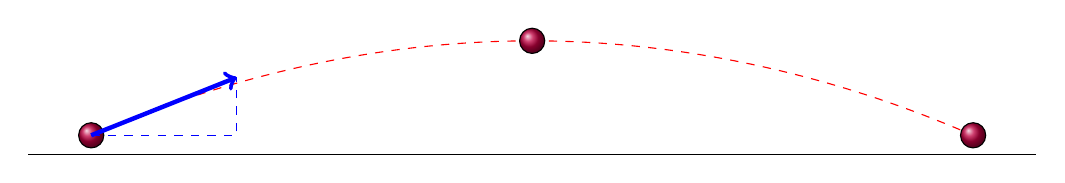
\begin{tikzpicture}[scale=0.8]
    \draw (-1,-0.3) -- ++(16,0);
  
    \draw[dashed,red] (7,1.5) parabola (0,0);
    \draw[dashed,red] (7,1.5) parabola (14,0);
  
    \draw[ball color=purple] (0,0) circle (0.2);
    \draw[ball color=purple] (7,1.5) circle (0.2);
    \draw[ball color=purple] (14,0) circle (0.2);
  
  
    \draw[dashed, blue] (0,0) -- (2.31,0) -- (2.31, 0.92);
    \draw[ultra thick, blue, ->] (0,0) -- (2.31, 0.92);
    %\draw[dashed, blue] (14,0) -- +(2.31,0) 
    %    -- +(2.31, -0.92);
    %\draw[ultra thick, blue, ->] (14,0) -- ++(2.31, -0.92);
  
  
    %\draw[ultra thick, blue, ->] (7,1.5) -- ++(2.31,0);
  \end{tikzpicture}
  
  \vspace{3em}
  
  
  \begin{parts}
    \part
      Calculate and label the initial resultant velocity.
    \part
      Calculate and label the velocity of the projectile at its maximum height.
    \part
      Calculate and label the resultant velocity the moment before the projectile hits the ground
      
  \end{parts}

  \vs 

\question
A car drives off a cliff at 15~m/s.  It falls until it has a $y$-velocity of 7~m/s.

  \begin{tikzpicture}
    
  \fill[gray] (3,.2)
      -- ++(0,1.8)
      -- ++(-2,0)
      -- ++(0,-1.8)
      -- cycle;
    \fill[white,pattern color=black, pattern= north east lines] (1,-.1) rectangle (7,.2);
    \draw[thick] (1,.2) -| (7,-.1);
    \draw[dashed,red] (3.1,2.3) parabola (6,.5);

    \draw[ultra thin, gray] (2,2.6) -- ++(-.3,0);
    \draw[ultra thin, gray] (1.9,2.4) -- ++(-.3,0);
    \draw[ultra thin, gray] (1.95,2.2) -- ++(-.4,0);

    \draw (2,2.1) pic[scale=0.2] {car};

  \end{tikzpicture}

  \vspace{3em}

  \begin{parts}
    \part
      Calculate and label the initial velocity.
    \part
      Calculate and label the resultant velocity the moment before the car hits the ground
      
  \end{parts}


  \vs
\end{questions}


\end{document}